% QUESTAO
Conforme a figura abaixo, o raio da circunfer\^encia circunscrita ao tri\^angulo \'e:

\parbox{0.24\linewidth}{

% ALTERNATIVAS
$4\sqrt{3}$
$4\sqrt{2}$
$8\sqrt{3}$
$8\sqrt{2}$
$8$

}\parbox{0.75\linewidth}{
\begin{center}
\vspace{-6mm}
\begin{tikzpicture}[rotate=71]
\def\legA{}
\def\legB{}
\def\legC{}
\triangulo
{$12$}	              {12}	               {60}
{}		  {13}	               {0}
{}	              {0}	               {0}
\circunferenciaCircunscrita
\end{tikzpicture}
\vspace{-6mm}
\end{center}
}


